#\section{Bewertungsmetriken}
https://ichi.pro/de/allgemeine-bewertungsmetriken-fur-die-regressionsanalyse-82886198762157

\subsection{Regression Analyse}
\subsubsection{Bestimmtheitsmaß $R^2$}
Gegeben eines Vektor $\Vector{Y}$ mit der Länge $n$, welcher als unabhängiger Teil eines Datensatzes eines Regressionsmodells fungiert, gibt es einen Vektor $\hat{\Vector{Y}}$, welcher die Vorhersagewerte zu jedem Datenpunkt $i$ beinhält. Ein \textit{Residualwert} ist $
\epsilon_i = y_i - \hat{y}_i$. Der \textit{Durchschnitt mean) der beobachteten Werte} wird definiert als $\overline{y}=\frac{1}{n}\sum y_i$. 
\begin{Definition}{Bestimmtheitsmaß}
	Sei $y_i$ beobachtet Werte $i\in \left\lbrace 1, \dots, n\right\rbrace$ der unabhängigen Variabel $Y$  eines Regressionsmodells. Sei $\hat{y}_i$ der geschätzte Werte für den gegeben Datensatz $i$.
	\begin{itemize}
		\item Die \gls{SQE} wird definiert durch 
		\begin{align}
			\text{SQE}:=\sum_i \epsilon_i = \sum_i (y_i - \hat{y}_i)^2 
		\end{align}
		\item Die \gls{SQT} wird definiert durch
		\begin{align}
			\text{SQT}:=\sum_i (y_i - \overline{y})^2
		\end{align}
		mit $\overline{y} = \frac{1}{n}\sum y_i$.
	\end{itemize} 
	Für das \textit{empirische Bestimmtheitsmaß} $R^2$ gilt
	\begin{align}
		R^2 := 1 - \frac{\gls{SQE}}{\gls{SQT}}
	\end{align}
\end{Definition}

\subsubsection{Mittlere Quadratische Abweichung}
Diese Bewertungsmetrik ist nicht mit der Standardabweichung zu wechseln. Diese ist ein Maß für die Streuung für eine Zufallsvariable, und wird auch \textit{Mittlere Quadratische Abweichung}
%TODO: Varianz Definition mit aufnehmen

Um die Verzerrung eines Punktschätzers kann mit Hilfe von \gls{MSE} bestimmt werden. 



- Root Mean Square Error (RMSE) $$RMSD= \sqrt{MSE(\hat{\theta})} = \sqrt{E((\hat{\theta}-\theta)^2)}$$
- Mean Absolute Error $$MAE = \frac{\Sigma |y_i - x_i|}{n}$$
\subsection{Klassifikation Analyse}
%TODO: Add to libary: https://divisbyzero.com/2008/09/22/what-is-the-difference-between-a-theorem-a-lemma-and-a-corollary/

% Verknüpfung von Definitionen, wo wird welche Definition benötigt

\section{Klassen eines statistischen Prozesses}
Das Merkmal (Variable) eines statistischen Prozesses lässt nach verschiedenen Kriterien klassifizieren.
\begin{description}
	\item[Anzahl der Ausprägungen] \: 
	\begin{itemize}
		\item Stetig
		\item Diskret
		\begin{itemize}
			\item abzählbar
			\item unendlich Ausprägungen
		\end{itemize} 
	\end{itemize}
	\item[Art der verwendeten Messskala/ Skalenniveau/ Messniveau] \:
	\begin{itemize}
		\item Nominalskala (Kategorial)
		\item Ordinalskala (Kategorial)
		\item Metrische Skala/ Kardianlskala
		\begin{itemize}
			\item Verhältnisskala
			\item Intervallskala
			\item Absolutskala
		\end{itemize} 	
	\end{itemize}
\end{description}

Variablen, die zur Gruppe das Skalenniveau Nominal und Ordninal aufwesen, können auch unter dem Begriff der \textbf{Kategorial Variable} gefasst werden. Das Skalenniveau gibt zum Ausdruck, welche Methoden/ Operationen auf eine bestimmt Variable durchgeführt werden kann. Der Begriff Skala gibt dabei zum Ausdruck, dass mit zunehmender Steigerung, mehr Operationen mit der Variable durchgeführt werden können. D. h., Variablen die in einem höheren Skalenniveau liegen, bieten eine größere Möglichkeit an Operationen.

\begin{figure}[H]
	\centering
	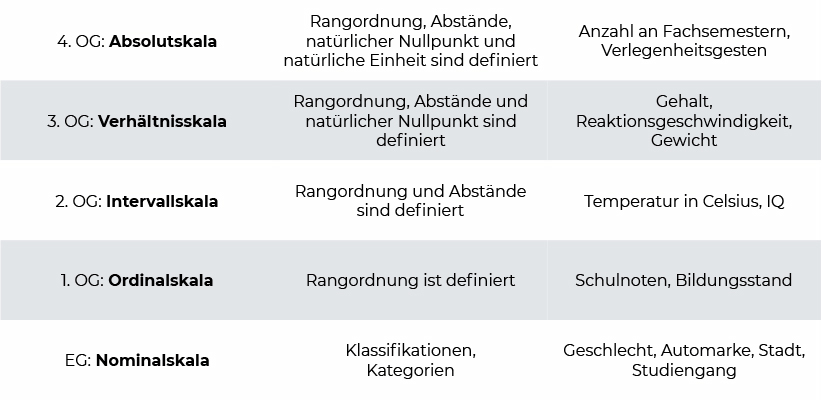
\includegraphics[scale = 0.4]{attachment/chapter_4/Scc023}
	\caption{Beispiele für Varialben unterschiedlicher Messskalas}
\end{figure}

\begin{figure}[H]
	\centering
	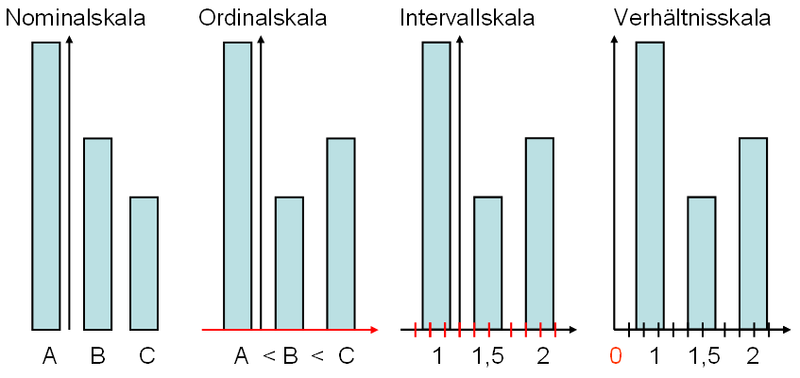
\includegraphics[scale = 0.37]{attachment/chapter_4/Scc024}
	\caption{Anordnungsmöglichkeiten für Ausprägungen von Variablen verschiedener Messkalas}
\end{figure}


